\chapter{Конструкторский раздел}
\label{cha:design}
В этом разделе будут рассмотрены требования к программе и схемы для реализации алгоритмов, математические расчёты.
Программа должна предоставлять возможность:
\begin{itemize}
	\item загружать модель мышц;
	\item визуализировать мышечные сокращения;
	\item задавать степень сокращения;
	\item изменять параметры загруженной модели;
\end{itemize}
\section{Общий алгоритм работы программы}
\label{sec:general}
Ниже приведён перечень основных этапов работы программы.
\begin{enumerate}
	\item Ожидание нажатия пользователем кнопки загрузки новой мышцы.
	\item Загрузка трёхмерной модели из файла.
	\item Задание пользователем параметров мышцы, а также степени её сокращения.
	\item Добавление модели в массив отображаемых объектов:
	\item Для всех полигонов модели:
	\begin{enumerate}
		\item Для каждого полигона: перевести в экранные координаты, вычислить интенсивность и глубину каждого пикселя, 
	\end{enumerate}
	\item Ожидание нажатия кнопки показа анимации сокращения.
	\item Построение анимации:
	\begin{enumerate}
		\item Формирование конечной модели на основе параметров мышцы.
		\item Установление соответствия между вершинами полигонов начального и конечного состояний.
		\item Интерполяция пути каждой вершины.
		\item Визуализировать каждое промежуточное состояние.
	\end{enumerate}
\end{enumerate}
На рисунках \ref{fig:01a-0} и \ref{fig:02a0} приведены IDEF0 диаграммы, представляющие организацию работы программы.
\begin{figure}
	\centering
	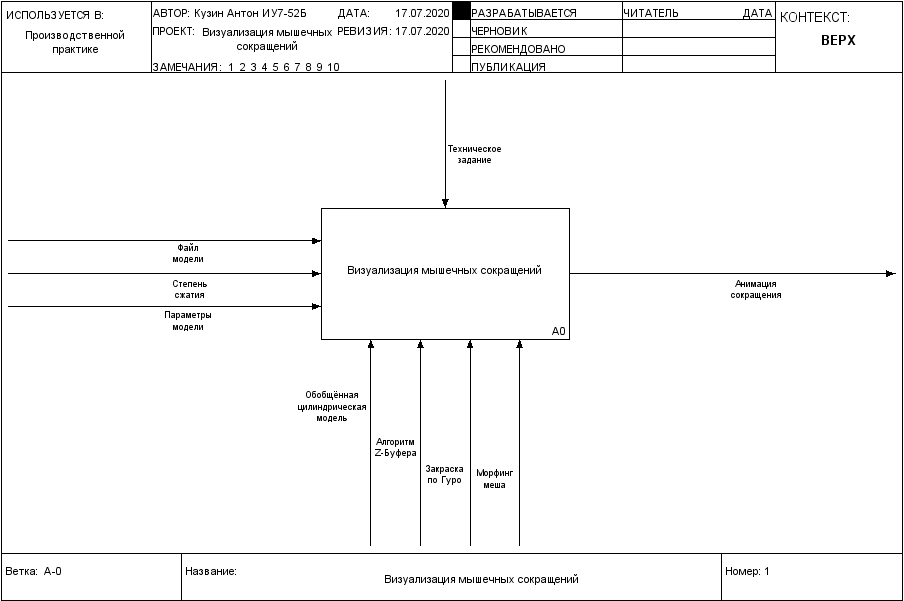
\includegraphics[width=\linewidth, angle=90]{01_A-0}
	\caption[IDEF0 диаграмма, блок А0]{IDEF0 диаграмма, блок А0}
	\label{fig:01a-0}
\end{figure}
\begin{figure}
	\centering
	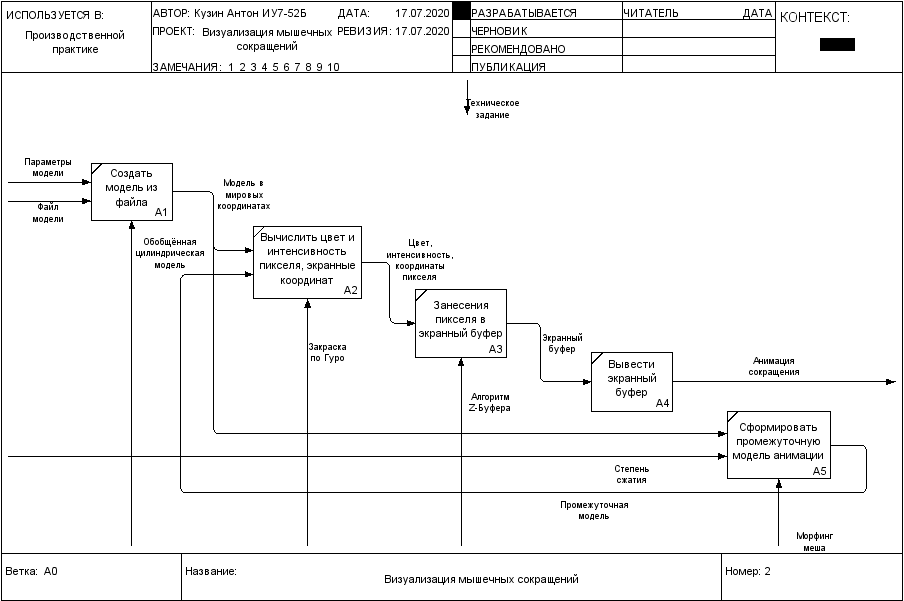
\includegraphics[width=0.7\linewidth]{02_A0}
	\caption[IDEF0 диаграмма, подробности работы блока А0]{IDEF0 диаграмма, подробности работы блока А0}
	\label{fig:02a0}
\end{figure}

\section{Реализуемые алгоритмы алгоритмы}
\label{sec:algs}
\paragraph{Алгоритм z-буфера}
в общем виде может быть описан последовательностью таких шагов:
\begin{enumerate}
	\item Заполнить буфер кадра фоновым значением интенсивности или цвета.
	\item Заполнить z-буфер минимальным значением z.
	\item Преобразовать каждый многоугольник в растровую форму в произвольном порядке:
	\begin{enumerate}
		\item Для каждого пикселя в многоугольнике вычислить его глубину z.
		\item Сравнить глубину z со значением z в буфере в этой же позиции. Если z > Zбуфер, то записать атрибут этого пикселя в буфер кадра и заменить Zбуфер на z.
	\end{enumerate}
\end{enumerate}

\paragraph{Простая модель освещения} интенсивность рассчитывается по закону Ламберта c учётом рассеянного освещения, представленного константой:
\begin{equation}\label{lambert2}
I = I_{a}k_{a} + I_{l}k_{d}\cos \theta \qquad 0\leq\theta\leq\pi/2
\end{equation}
$I$ - интенсивность отражённого света, $I_{i}$ - интенсивность точечного источника, $k_{d}$ - коэффициент диффузного отражения ($0\leq k_{d}\leq 1$), $\theta$ - угол между направлением света и нормалью к поверхности, $I_{a}$ - интенсивность рассеянного света, $k_{a}$ - коэффициент диффузного отражения ($0\leq k_{a}\leq 1$).

\paragraph{Закраска методом Гуро} интенсивность в точке определяется линейной интерполяцией интенсивности в точках пересечения сканирующей строки с рёбрами треугольника. Чтобы получить значение в этих точках необходимо интерполировать интенсивность в вершинах, соединяемых этими рёбрами:
\begin{equation}
I_{inter}=uI_{A}+(1-u)I_{B} \qquad 0\leq u \leq 1
\end{equation}
где u - отношение расстояний от точки пересечения до вершин.

\paragraph{Морфинг меша} можно разделить на два этапа: установление соответствия между полигонами начального и конечного состояний модели и интерполяция положения вершин. На рисунке \ref{fig:morphingalg} представлен алгоритм морфинга мешей с методом сортировки рёбер для установления соответствия между рёбрами.
\begin{figure}
	\centering
	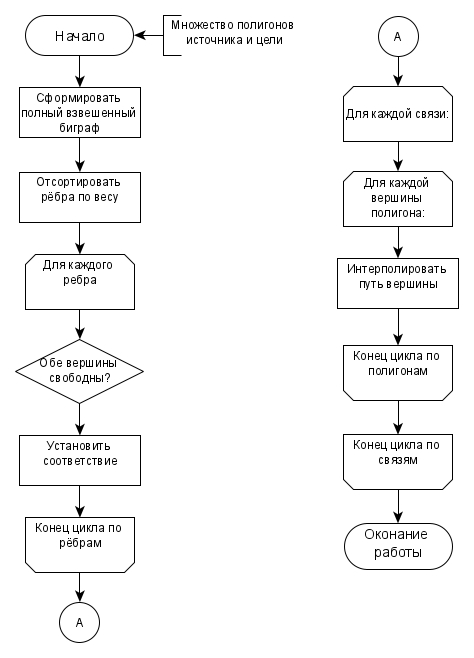
\includegraphics[width=0.7\linewidth]{morph}
	\caption[Алгоритм морфинга]{Алгоритм морфинга}
	\label{fig:morphingalg}
\end{figure}
